\documentclass{article}
\usepackage{subcaption}
\usepackage{circuitikz}
\usepackage{graphicx} % Required for inserting images
\usepackage[absolute,overlay]{textpos}
\usepackage{float} % H placement
\usepackage{amsmath}
\usepackage{amssymb}
\usepackage[a4paper, left=2.5cm, right=2.5cm, top=2.5cm, bottom=2.5cm]{geometry}
\usepackage{listings}           % Code listing support
\usepackage{xcolor}             % Color for syntax highlighting
\usepackage{tikz}
\usetikzlibrary{automata, positioning, arrows, calc}
\tikzset{
    ->, 
    >=stealth,
    shorten >=2pt, shorten <=2pt,
    node distance=2.8cm,
    every state/.style={draw=blue!55,very thick,fill=blue!20},
    initial text=$ $,
}
\usepackage[colorlinks=true,
            linkcolor=black,
            citecolor=blue,
            urlcolor=blue]{hyperref}

% C/Arduino listing style configuration
\lstdefinestyle{cpp}{
    language=C++,
    basicstyle=\footnotesize\ttfamily,
    keywordstyle=\color{blue}\bfseries,
    commentstyle=\color{green!60!black}\itshape,
    stringstyle=\color{red},
    numbers=left,
    numberstyle=\tiny\color{gray},
    stepnumber=1,
    numbersep=8pt,
    showspaces=false,
    showstringspaces=false,
    showtabs=false,
    frame=single,
    rulecolor=\color{black},
    tabsize=4,
    captionpos=b,
    breaklines=true,
    breakatwhitespace=false,
}

\title{IoT -- Smart Trash Bin}
\author{Anders Falkesgaard (s245905), Andreas Jacobsen (s241123)
\\Jonas Beck Jensen (s240324), Mads Rudolph (s246132)
\\Sigurd Hestbech Christiansen (s245534), Tobias Nilsson (s233987)}
\date{May 2026}

\newcommand{\mainfile}{}
\newcommand{\doubleunderline}[1]{\underline{\underline{#1}}}

\begin{document}

% ============================================================
%  FRONT PAGE
% ============================================================

% Logo in top right
\begin{textblock*}{3cm}(17.5cm,1cm)
  
\includegraphics[scale=0.5]{images/frontpage/dtu_logo.png}
\end{textblock*}

\maketitle

\begin{center}
     \textbf{Course 34315 -- IoT application and infrastructure implementation}
\end{center}

\vspace*{0cm}
\begin{figure}
    \vspace{-6cm}
    \hspace{-2cm}
    
\includegraphics[width=1.0\linewidth]{images/frontpage/dtu_retning.png}
    \label{fig:frontpage}
\end{figure}

% --- Row 1: Andreas, Jonas, Mads ---
\begin{textblock*}{8cm}(2.5cm,9cm)
    \fbox{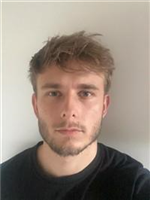
\includegraphics[scale=0.5]{images/frontpage/dtu_andreas.png}}
\end{textblock*}
\begin{textblock*}{8cm}(2.5cm,12cm)
    \textbf{Andreas}
\end{textblock*}
\begin{textblock*}{8cm}(2.5cm,12.4cm)
    \textbf{s241123}
\end{textblock*}

\begin{textblock*}{8cm}(8.3cm,9cm)
    \fbox{
\includegraphics[scale=0.26]{images/frontpage/dtu_jonas.png}}
\end{textblock*}
\begin{textblock*}{8cm}(8.3cm,12cm)
    \textbf{Jonas}
\end{textblock*}
\begin{textblock*}{8cm}(8.3cm,12.4cm)
    \textbf{s240324}
\end{textblock*}

\begin{textblock*}{8cm}(14.1cm,9cm)
    \fbox{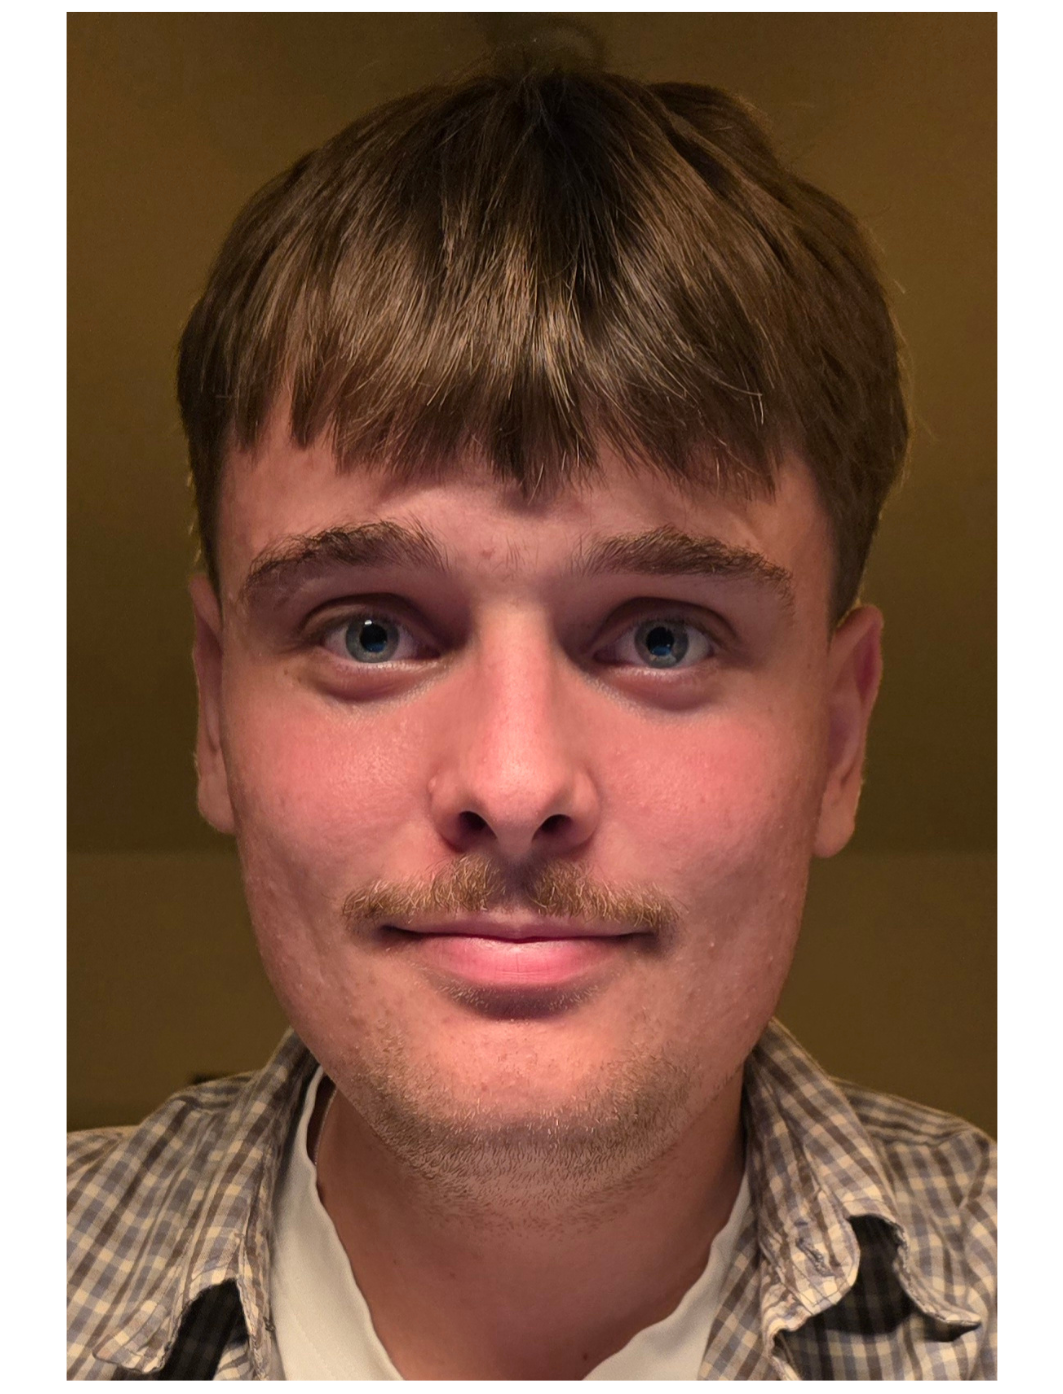
\includegraphics[scale=0.23]{images/frontpage/dtu_mads.png}}
\end{textblock*}
\begin{textblock*}{8cm}(14.1cm,12cm)
    \textbf{Mads}
\end{textblock*}
\begin{textblock*}{8cm}(14.1cm,12.4cm)
    \textbf{s246132}
\end{textblock*}

% --- Row 2: Sigurd, Anders, Tobias ---
\begin{textblock*}{8cm}(2.5cm,13cm)
    \fbox{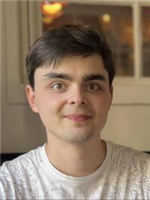
\includegraphics[scale=0.5]{images/frontpage/dtu_sigurd.png}}
\end{textblock*}
\begin{textblock*}{8cm}(2.5cm,16cm)
    \textbf{Sigurd}
\end{textblock*}
\begin{textblock*}{8cm}(2.5cm,16.4cm)
    \textbf{s245534}
\end{textblock*}

\begin{textblock*}{8cm}(8.3cm,13cm)
    \fbox{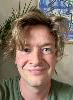
\includegraphics[width=2.6cm]{images/frontpage/dtu_anders.png}}
\end{textblock*}
\begin{textblock*}{8cm}(8.3cm,16cm)
    \textbf{Anders}
\end{textblock*}
\begin{textblock*}{8cm}(8.3cm,16.4cm)
    \textbf{s245905}
\end{textblock*}

\begin{textblock*}{8cm}(14.1cm,13cm)
    \fbox{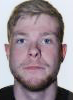
\includegraphics[width=2.6cm]{images/frontpage/dtu_tobias.png}}
\end{textblock*}
\begin{textblock*}{8cm}(14.1cm,16cm)
    \textbf{Tobias}
\end{textblock*}
\begin{textblock*}{8cm}(14.1cm,16.4cm)
    \textbf{s233987}
\end{textblock*}

\vspace{9cm}
\begin{center}
     \textbf{\large Group 16}
\end{center}

% ============================================================
%  CONTENTS
% ============================================================
\newpage
\tableofcontents
\newpage

% ============================================================
%  10-PAGE PROJECT BRIEF
% ============================================================
\ifdefined\mainfile\else
\documentclass{article}
\usepackage{graphicx}
\usepackage{float}
\usepackage{amsmath}
\usepackage{amssymb}
\usepackage[a4paper, left=2.5cm, right=2.5cm, top=2.5cm, bottom=2.5cm]{geometry}
\usepackage[colorlinks=true,linkcolor=black,citecolor=blue,urlcolor=blue]{hyperref}
\begin{document}
\fi

\section{Executive summary}
\label{sec:executive-summary}

This project presents the design and construction of a smart, self‑closing trash bin with logging and administrative features. The system automates the sealing of trash bags while collecting and displaying usage data, aiming to reduce the everyday issues of overflowing kitchen bins and forgotten bag inventory.
\\ \\
\noindent
A scaled‑down prototype was developed at a 1:2 scale and integrates both hardware and software components typical of an IoT system. The physical solution includes an automated bag‑closing mechanism driven by electric motors and controlled by an ESP8266, supported by sensors for monitoring trash level and system state. An on‑device display provides the user with status information and system feedback.
\\ \\
\noindent
In addition, a web application was developed to log data related to remaining trash bags and to present real‑time information, such as how full the current trash bag is. Overall, the project demonstrates how IoT technology can combine physical automation with cloud‑based data logging and user‑friendly monitoring.

\ifdefined\mainfile\else
\end{document}
\fi

\ifdefined\mainfile\else
\documentclass{article}
\usepackage{graphicx}
\usepackage{float}
\usepackage{amsmath}
\usepackage{amssymb}
\usepackage[a4paper, left=2.5cm, right=2.5cm, top=2.5cm, bottom=2.5cm]{geometry}
\usepackage[colorlinks=true,linkcolor=black,citecolor=blue,urlcolor=blue]{hyperref}
\begin{document}
\fi

\section{Pain -- the problem we solve}
\label{sec:pain}

This project was developed to assist individuals who may have difficulty managing their household waste, such as elderly or disabled users, as well as to support people who may forget to empty their trash bins regularly.\\
The system consists of a smart trash bin capable of monitoring the fill level in real time. When the bin reaches 80\% capacity, it automatically seals the trash bag, improving both convenience and hygiene. This feature reduces the need for manual handling, making the solution more accessible for users with limited mobility.\\
In addition, the system provides remote monitoring functionality, allowing users to check the current status of the trash bin and track the number of remaining trash bags in their inventory.\\
The smart bin is integrated with the IFTTT platform, enabling push notifications to be sent directly to the user. These notifications alert the user when the trash bag needs to be emptied or when the number of available bags falls below three. This ensures timely maintenance and helps prevent the user from running out of necessary supplies.


\ifdefined\mainfile\else
\end{document}
\fi

\ifdefined\mainfile\else
\documentclass{article}
\usepackage{graphicx}
\usepackage{float}
\usepackage{amsmath}
\usepackage{amssymb}
\usepackage[a4paper, left=2.5cm, right=2.5cm, top=2.5cm, bottom=2.5cm]{geometry}
\usepackage[colorlinks=true,linkcolor=black,citecolor=blue,urlcolor=blue]{hyperref}
\begin{document}
\fi

\section{Solution}
\label{sec:solution}

Our solution is a connected trash bin that closes its own bag and reports its status to a phone-friendly web dashboard. Internally the system has four parts that never talk to each other directly:

\begin{itemize}
    \item \textbf{ESP8266 in the bin} -- runs a state machine, reads sensors, drives the closure mechanism and pushes data to the cloud.
    \item \textbf{ThingSpeak cloud channel} -- the shared noticeboard. The ESP and the dashboard both read from and write to the same numbered fields.
    \item \textbf{Web dashboard} (\url{https://dtutrash.netlify.app/}) -- a single static HTML page that shows live bin status and lets the user reset the bag inventory.
    \item \textbf{IFTTT push notifications} -- triggered by ThingSpeak React rules when a bag-full event fires or when the bag stock runs low.
\end{itemize}
\noindent
\textbf{Instructions for use.} After mounting a new bag, the user presses the reset button. The bin then enters its \textsc{check} state and silently monitors the fill level using an ultrasonic sensor. When the distance from the sensor down to the trash drops below 8\,cm (\textasciitilde 80\% full), the bin enters its \textsc{close} state: two stepper motors pulls the plastic strings attached to the bag, closing the bag. The bin then enters \textsc{empty\_me} and pushes a notification to the user's phone. After the user replaces the bag and presses reset, the cycle starts over. The OLED display on the bin shows the current state so the user knows what is happening without checking their phone.
\newpage
Figure~\ref{fig:state-diagram} summarises the device-side state machine.

%\begin{figure}[H]
%    \centering
%    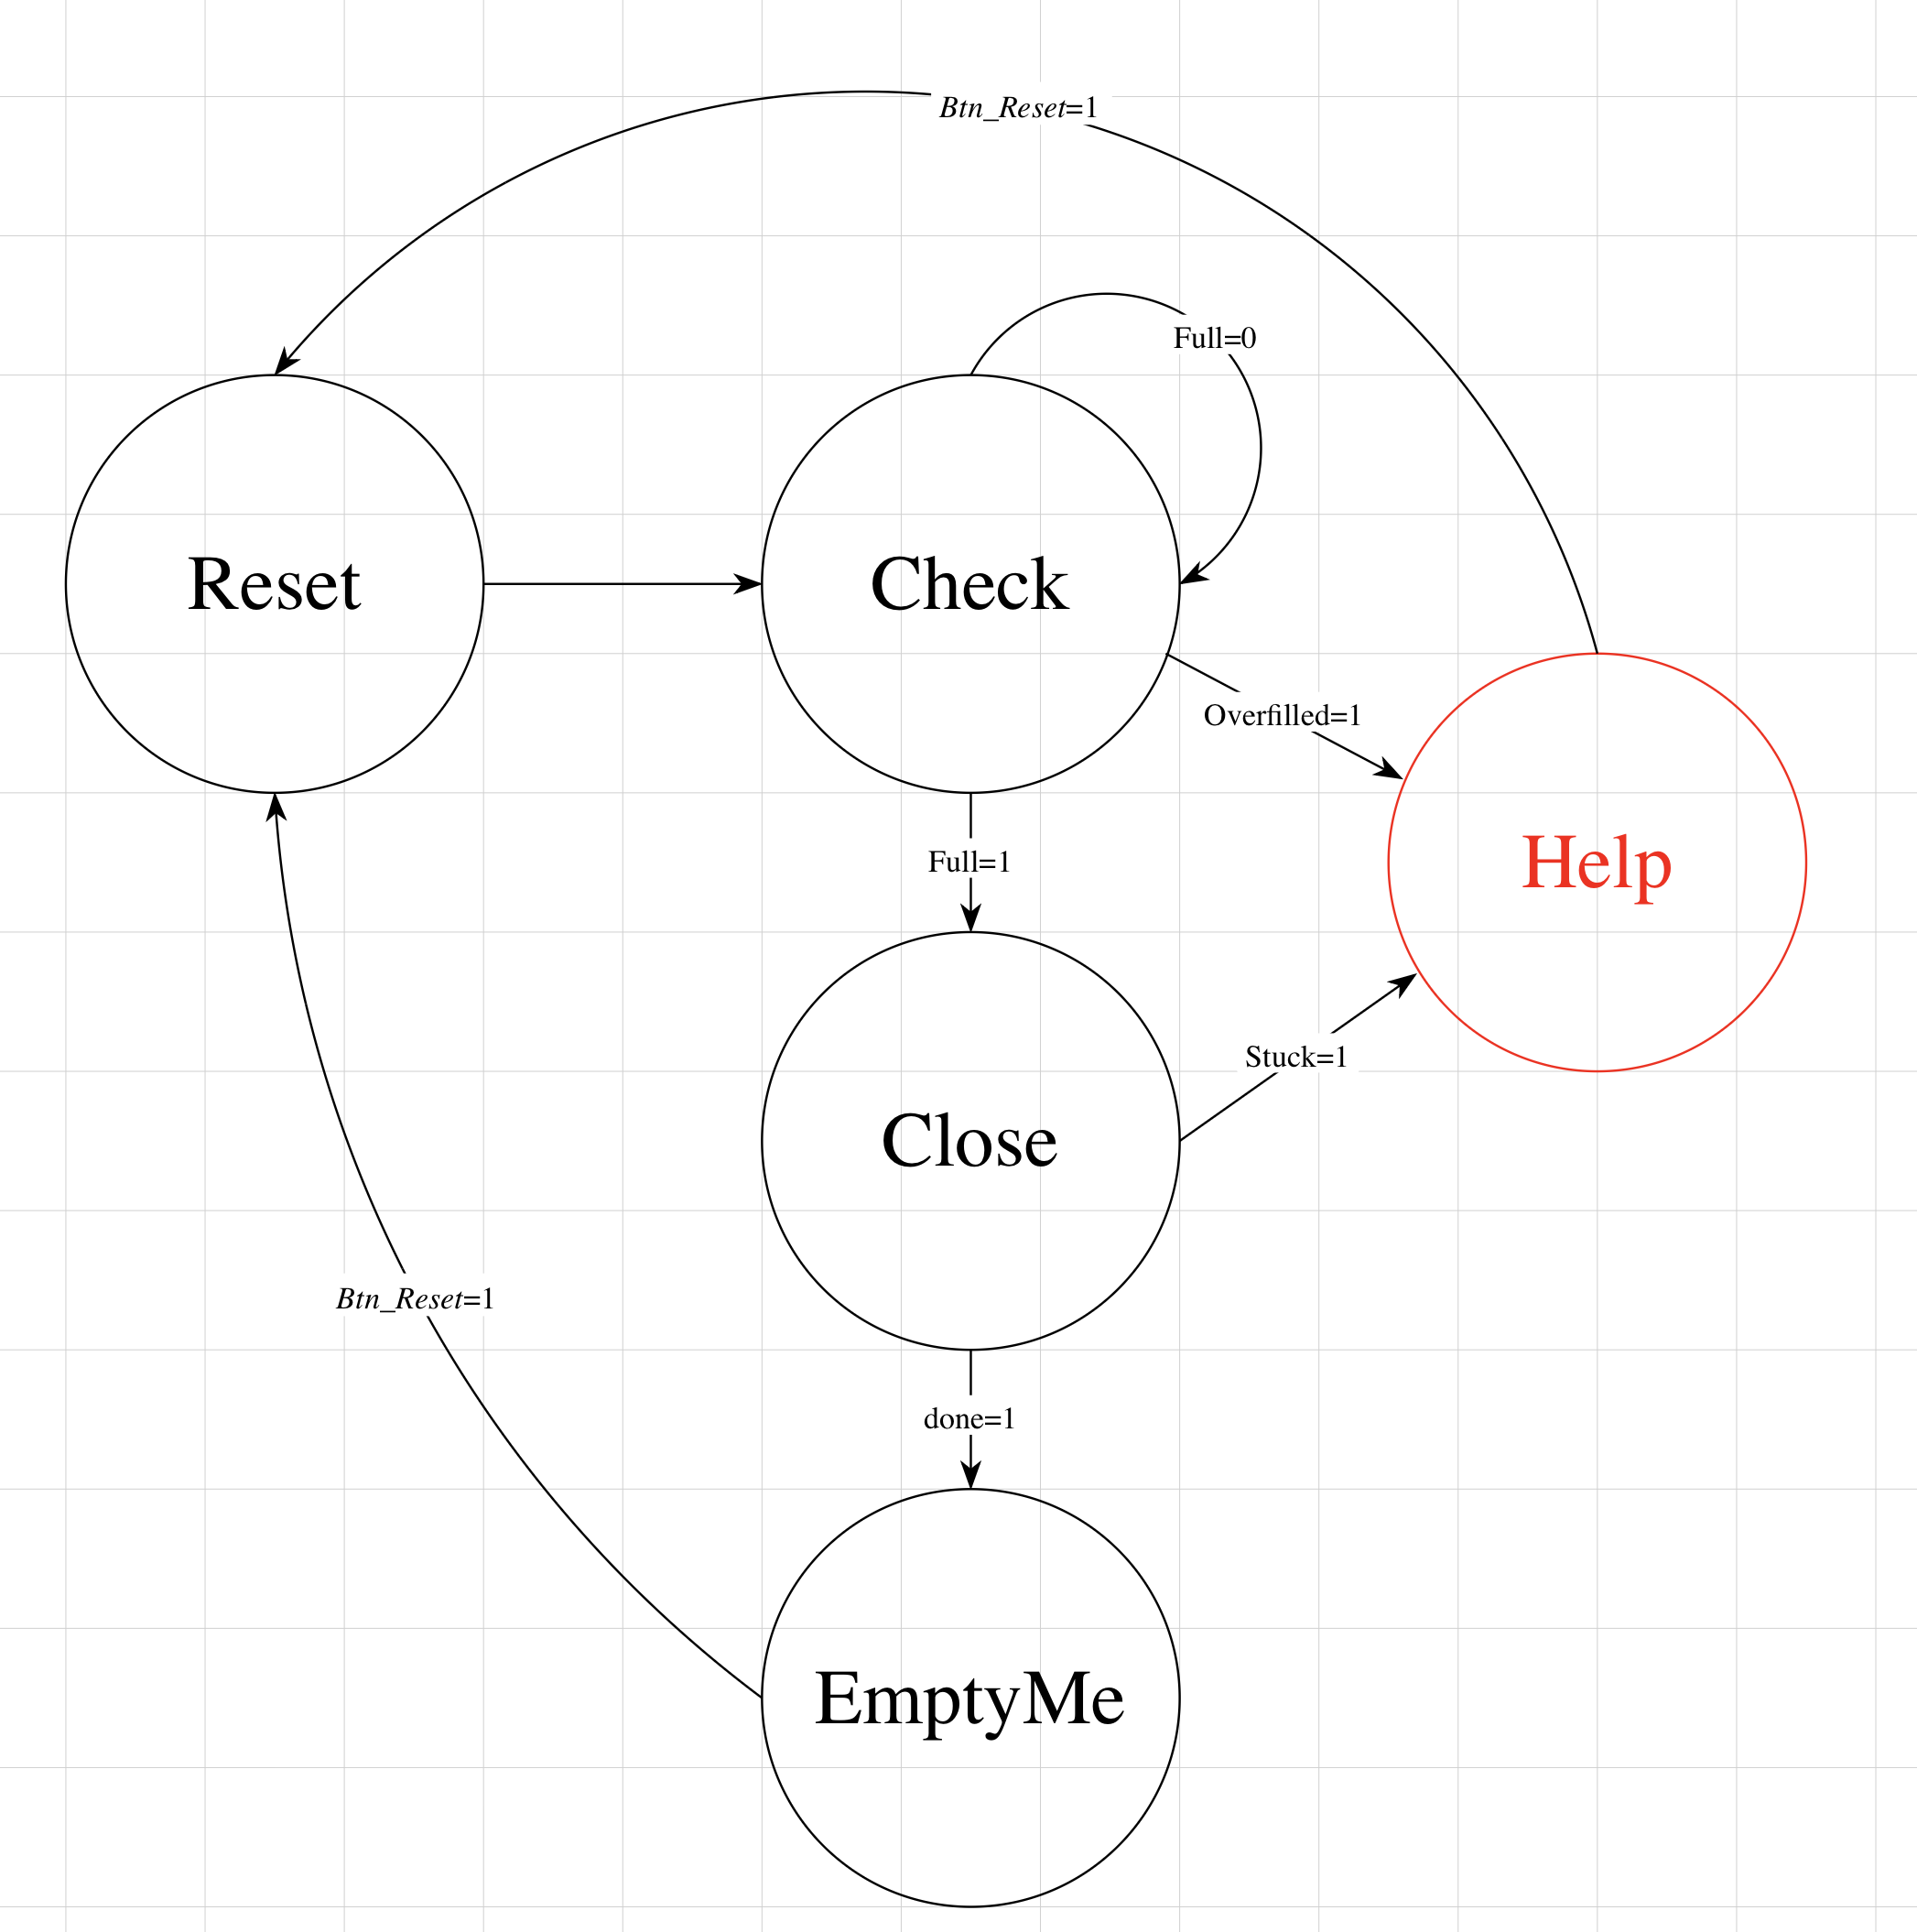
\includegraphics[width=0.6\linewidth]{images/system/state_diagram.png}
%    \caption{Device-side state machine. \textsc{reset} initialises the system after a bag is replaced. \textsc{check} polls the ultrasonic sensor; on \texttt{Full=1} it transitions to \textsc{close}, which drives the stepper motors and pushes a bag-full event. \textsc{emptyme} waits for the user to reset. \textsc{help} is an error state reached on overfill or stuck-motor conditions.}
%    \label{fig:state-diagram}
%\end{figure}


\ifdefined\mainfile\else
\end{document}
\fi

\ifdefined\mainfile\else
\documentclass{article}
\usepackage{graphicx}
\usepackage{float}
\usepackage{amsmath}
\usepackage{amssymb}
\usepackage[a4paper, left=2.5cm, right=2.5cm, top=2.5cm, bottom=2.5cm]{geometry}
\usepackage[colorlinks=true,linkcolor=black,citecolor=blue,urlcolor=blue]{hyperref}
\begin{document}
\fi

\subsection{Hardware design}
\label{sec:hardware}

The brain of the bin is an \textbf{ESP8266 NodeMCU} module - it has Wifi-capabilities, which allows us to run the intended program. It was not, the ideal candidate: the ESP8266 only exposes a handful of usable GPIO pins and several of those have boot-time roles, which made the pin layout one of the recurring headaches of the project. However we manged to keep the entire system limited to a single ESP-unit, making the system cheaper to produce and sell.
\\ \\
Around the ESP we built up the rest of the hardware listed in Table~\ref{tab:components}. The selection satisfies the course's component requirements -- one analog sensor (LM35), one digital sensor (HC-SR04), one form of actuation (the steppers) and an on-device display (the OLED).

\begin{table}[H]
    \centering
    \begin{tabular}{l|l|l}
        \textbf{Component} & \textbf{Role} & \textbf{Type} \\
        \hline
        ESP8266 NodeMCU                 & WiFi MCU                & Microcontroller \\
        HC-SR04 ultrasonic sensor       & Fill level measurement  & \textbf{Digital} sensor \\
        LM35 temperature sensor         & Temperature measurement & \textbf{Analog} sensor \\
        28BYJ-48 stepper motor (x2)     & Bag closure mechanism   & \textbf{Actuator} \\
        ULN2003 driver board (x2)       & Stepper coil driver     & Driver \\
        SSD1306 OLED display (I\textsuperscript{2}C, 0.96\textquotedbl) & Local status display & Display \\
        Push button                     & User reset              & Input \\
    \end{tabular}
    \caption{Components used in the Smart Trash Bin}
    \label{tab:components}
\end{table}
\noindent
Power is supplied from a battery and convertet down to 5\,V. The ESP8266 runs from its onboard 3.3\,V regulator, while the stepper drivers and the OLED share the 5\,V rail. The HC-SR04 outputs 5\,V on its Echo line, so it is divided down with a 1\,k$\Omega$/2\,k$\Omega$ resistor pair before reaching a 3.3\,V-only GPIO. The full pinout is listed in Table~\ref{tab:pinout}, and a larger circuit diagram is reproduced in the appendix.

\begin{table}[H]
    \centering
    \begin{tabular}{l|l|l}
        \textbf{Component} & \textbf{ESP8266 pin} & \textbf{Note} \\
        \hline
        HC-SR04 Trig     & D5  & digital output \\
        HC-SR04 Echo     & D6  & digital input (1k/2k divider) \\
        ULN2003 IN1      & D8  & stepper coil 1 \\
        ULN2003 IN2      & D7  & stepper coil 2 \\
        ULN2003 IN3      & D2  & stepper coil 3 (shared with I\textsuperscript{2}C SDA) \\
        ULN2003 IN4      & D0  & stepper coil 4 (moved from D1 to free SCL) \\
        SSD1306 SDA      & D2  & I\textsuperscript{2}C data \\
        SSD1306 SCL      & D1  & I\textsuperscript{2}C clock \\
        LM35 Vout        & A0  & analog input, 10-bit ADC \\
        Reset button     & D3  & digital input, internal pull-up \\
    \end{tabular}
    \caption{Pinout for the ESP8266 module}
    \label{tab:pinout}
\end{table}
\noindent
\noindent To check whether the bin could run without mains power we made a small power budget in MATLAB. The script sums the current drawn by the ESP8266, the OLED, the two sensors and the stepper driver, weights each by how long the bin spends in every state over a day, and includes the loss in the buck converter. Comparing a 9\,V alkaline battery with a pair of 18650 Li-ion cells, it shows that the alkaline option lasts well under a day with the WiFi always on, while the Li-ion pack lasts considerably longer, and that a modem-sleep or light-sleep mode would extend this further. Deep sleep was left out on purpose, since on the ESP8266 it resets the chip on wake and would lose the state machine.
\begin{align*}
Total_{Power} &= V_{5\text{V}}\ I_{\text{avg}} & I_{\text{avg}} &= \frac{1}{T}\sum_{s} I_{s}\, t_{s} \\
I_{\text{batt}} &= \frac{Total_{Power}}{\eta\, V_{\text{batt}}} + I_{q} & t_{\text{life}} &= \frac{Q_{\text{batt}}}{I_{\text{batt}}}
\end{align*}
\noindent where $I_{s}$ and $t_{s}$ are the average current and the time spent in state $s$ over one day $T$, $V_{5\text{V}}$ is the rail voltage, $\eta$ the buck-converter efficiency, $I_{q}$ the buck quiescent current, and $Q_{\text{batt}}$ and $V_{\text{batt}}$ the battery charge and nominal voltage.
\noindent The graphs for the power calculations, can be found on the poster.
\ifdefined\mainfile\else
\end{document}
\fi

\ifdefined\mainfile\else
\documentclass{article}
\usepackage{graphicx}
\usepackage{float}
\usepackage{amsmath}
\usepackage{amssymb}
\usepackage[a4paper, left=2.5cm, right=2.5cm, top=2.5cm, bottom=2.5cm]{geometry}
\usepackage[colorlinks=true,linkcolor=black,citecolor=blue,urlcolor=blue]{hyperref}
\begin{document}
\fi

\section{Communication technologies}
\label{sec:comms}

\subsection{WiFi (IEEE 802.11 b/g/n)}
\label{sec:wifi}

The bin connects to the home network over standard 2.4\,GHz WiFi, exposed by the ESP8266's built-in radio. WiFi uses CSMA/CA channel access on the unlicensed ISM band and provides per-link symmetric encryption (WPA2/WPA3). At link level the ESP8266 supports raw data rates from 1\,Mb/s up to 72.2\,Mb/s; in practice the limiting factor for our use case is the cloud round-trip, not the air link.

We chose WiFi (rather than e.g. BLE, LoRaWAN or Zigbee) for three reasons. First, the course explicitly requires it. Second, every household with a kitchen already has WiFi infrastructure, so the bin is plug-and-play. Third, WiFi is high-bandwidth and IP-routable, which means we can talk directly to any HTTP endpoint on the public internet (ThingSpeak) without needing a gateway.

\textbf{Pros.} Ubiquitous in homes; no extra gateway needed; high bandwidth; native IP stack so we can use ordinary HTTP REST calls.\\
\textbf{Cons.} Higher power consumption than BLE/LoRa, especially while the radio is active; depends on the user's home AP being reachable; 2.4\,GHz band can be noisy (microwaves, neighbours' APs).

\subsection{HTTP REST over the public internet}
\label{sec:http}

All cloud communication uses unencrypted HTTP GET requests against the ThingSpeak API. ThingSpeak is a simple cloud database with eight numbered fields per channel; writing a sample is a single URL fetch, and reading the most recent samples is another. Both the ESP and the dashboard speak the same protocol, so the integration code is symmetric.

\textbf{Pros.} Trivially simple; works from anything that can open a URL; ThingSpeak's free tier is sufficient for our cadence.\\
\textbf{Cons.} Plain HTTP, no encryption (acceptable for non-sensitive telemetry but not for production); each push is a full TCP+HTTP round-trip, which is heavy compared to a long-lived MQTT session.

\subsection{ThingSpeak React + IFTTT webhooks}
\label{sec:react}

ThingSpeak's \emph{React} feature watches a field for a condition (\texttt{field4 = 1} or \texttt{field2 < 3}) and fires a webhook URL when it triggers. The webhook target is an IFTTT applet, which in turn delivers a push notification to the IFTTT app on the user's phone.

\textbf{Pros.} No notification server of our own to maintain; native iOS/Android notifications; rules are configured in a browser without touching firmware.\\
\textbf{Cons.} Adds a hop (so notifications arrive with a few seconds of extra latency); free-tier React has a minimum 15-minute re-trigger interval; both services can change their APIs without warning.

\ifdefined\mainfile\else
\end{document}
\fi

\ifdefined\mainfile\else
\documentclass{article}
\usepackage{graphicx}
\usepackage{float}
\usepackage{amsmath}
\usepackage{amssymb}
\usepackage[a4paper, left=2.5cm, right=2.5cm, top=2.5cm, bottom=2.5cm]{geometry}
\usepackage[colorlinks=true,linkcolor=black,citecolor=blue,urlcolor=blue]{hyperref}
\begin{document}
\fi

\section{Software design}
\label{sec:software}

The software has three layers: firmware on the ESP8266, the ThingSpeak cloud channel that mediates between everyone, and the static web dashboard hosted on Netlify. Each layer is independent -- if any one is restarted, the others keep working.

\subsection{Firmware architecture (ESP8266)}
\label{sec:firmware}

The firmware is written in Arduino C++ and built around an explicit state machine. The main loop dispatches on a \texttt{State} variable and the four normal states (\textsc{load}, \textsc{check}, \textsc{close}, \textsc{empty\_me}) are joined by an error state (\textsc{help}) for overfill and stuck-motor conditions. Three independent concerns run alongside the state machine:

\begin{itemize}
    \item \textbf{Sensor sampling.} The HC-SR04 is read by sending a 10\,$\mu$s trigger pulse and timing the echo with \texttt{pulseIn()}; distance is converted using the speed of sound ($d = t \cdot 0.0343 / 2$ cm). The LM35 is sampled through the ESP's 10-bit ADC with the reference calibrated to 2.667\,V, and the raw reading is smoothed with an IIR filter (10-sample running mean blended 30/70 with the previous value).
    \item \textbf{ThingSpeak push.} A non-blocking timer pushes fields 1--4 and 6 every 16\,s when data has changed (the free-tier minimum is 15\,s between writes).
    \item \textbf{ThingSpeak poll.} A separate timer polls field 5 (the bag-count command from the dashboard) every 30\,s, leaving CPU headroom for the state machine.
\end{itemize}

To save power between pushes the WiFi radio is dropped into light-sleep, which cuts idle current significantly while still allowing the ESP to wake on a timer.

\subsection{Cloud layer (ThingSpeak)}
\label{sec:cloud}

ThingSpeak channel 3364403 acts as the single source of truth. Six of its eight fields are in use; the mapping is shown in Table~\ref{tab:fields}.

\begin{table}[H]
    \centering
    \begin{tabular}{c|l|l|l}
        \textbf{Field} & \textbf{Meaning} & \textbf{Written by} & \textbf{Read by} \\
        \hline
        1 & Distance (cm) from ultrasonic sensor & ESP & Dashboard \\
        2 & Bags remaining                       & ESP & Dashboard, IFTTT React \\
        3 & State (0=LOAD, 1=CHECK, 2=CLOSE, 3=EMPTY\_ME) & ESP & Dashboard \\
        4 & Bag-full event (1 = full)            & ESP & IFTTT React \\
        5 & Set-bag-count command                & Dashboard & ESP \\
        6 & Temperature (\textdegree C) from LM35 & ESP & Dashboard \\
    \end{tabular}
    \caption{ThingSpeak field map}
    \label{tab:fields}
\end{table}

\subsection{Dashboard (static HTML on Netlify)}
\label{sec:dashboard}

The dashboard at \url{https://dtutrash.netlify.app/} is a single HTML file (\texttt{docs/index.html}) of plain HTML/CSS/JavaScript -- no framework, no backend, no build step. Netlify just serves the file. The page calls the ThingSpeak feeds endpoint on a 5\,s timer, picks the most recent entry that actually contains ESP data (ignoring entries that only set field 5) and updates the cards. A POST-style write goes back the other way when the user clicks Save on the bag-count input.

\subsection{Code, libraries and source}
\label{sec:code}

All firmware and dashboard code is in the project repository on GitHub. Third-party libraries used:

\begin{itemize}
    \item \texttt{ESP8266WiFi}, \texttt{ESP8266HTTPClient}, \texttt{ESP8266WebServer} -- WiFi and HTTP client (built into the ESP8266 Arduino core).
    \item \texttt{Stepper} (Arduino built-in) -- driving the 28BYJ-48 motors.
    \item \texttt{Adafruit\_GFX} + \texttt{Adafruit\_SSD1306} -- OLED rendering.
    \item ThingSpeak HTTP REST API -- no client library; we issue raw \texttt{http.GET()} calls.
\end{itemize}

The submitted DTU LEARN bundle includes the complete Arduino sketch (\texttt{sketch\_apr16a.ino}) and the dashboard source (\texttt{docs/index.html}), as well as IFTTT/ThingSpeak React configuration screenshots so the cloud-side configuration is reproducible.

\ifdefined\mainfile\else
\end{document}
\fi

\ifdefined\mainfile\else
\documentclass{article}
\usepackage{graphicx}
\usepackage{float}
\usepackage{amsmath}
\usepackage{amssymb}
\usepackage[a4paper, left=2.5cm, right=2.5cm, top=2.5cm, bottom=2.5cm]{geometry}
\usepackage[colorlinks=true,linkcolor=black,citecolor=blue,urlcolor=blue]{hyperref}
\begin{document}
\fi

\section{How we present data to the user}
\label{sec:presentation}

The user sees information about the bin in three different places, each chosen for a different context.

\subsection{The web dashboard}
\label{sec:dashboard-ui}

The primary surface is the dashboard at \url{https://dtutrash.netlify.app/}. It is intentionally a single page with four large cards -- \emph{Bags remaining}, \emph{Distance}, \emph{State} and \emph{Temperature} -- so the user can glance at it on their phone and immediately understand the bin's status. The page auto-refreshes every 5 seconds.

Two small UX details are worth calling out because they cost real effort to get right:

\begin{itemize}
    \item \textbf{ONLINE/OFFLINE pill.} The pill in the top-right corner is not based on HTTP success -- ThingSpeak will happily serve cached data when the ESP is unplugged. Instead the dashboard checks the age of the latest ESP reading: if it is older than 90\,s (three times the ESP's polling cycle), the pill flips to OFFLINE. This honestly reflects whether the bin is alive.
    \item \textbf{Filtering out command-only entries.} When the user writes a new bag count, ThingSpeak creates a new entry where \texttt{field5} is set but \texttt{field1/2/3} are \texttt{null}. If the dashboard simply showed the latest entry it would briefly display \texttt{--} for distance and bags. Instead it pulls the 10 most recent entries and walks backwards to find the latest one with \texttt{field1 != null}.
\end{itemize}

The dashboard also has a single input box and a Save button to set the bag inventory remotely. The flow is: the dashboard writes the desired count to field 5; the ESP polls field 5 within 30\,s, copies it into its internal counter, and confirms by writing the new value back to field 2 on the next push. The dashboard then sees field 2 update on its next refresh. Worst-case round-trip is approximately $30 + 16 + 5 = 51$ s, which we communicate to the user with a toast that says "Set to X bags -- ESP fetches in $<$30\,s".

\subsection{The on-device OLED}
\label{sec:oled}

A 0.96\,\textquotedbl\ SSD1306 OLED on the lid shows the current FSM state in plain English (\textsc{Ready}, \textsc{Checking}, \textsc{Closing bag}, \textsc{Replace bag}) plus the current bag inventory and the latest temperature reading. This is the channel for moments when the user is actually standing at the bin and does not want to pull out their phone.

\subsection{Push notifications}
\label{sec:notifications}

For asynchronous alerts -- "your bag is full" or "you are running out of bags" -- the system pushes through IFTTT. The user does not need any app of ours installed; they only need IFTTT, which most households already have for other automations. Two notifications are configured:

\begin{itemize}
    \item \emph{Trash bag is full -- please replace it} (triggered by \texttt{field4 = 1}).
    \item \emph{Running low on trash bags} (triggered by \texttt{field2 $<$ 3}).
\end{itemize}

This three-channel split -- live dashboard for monitoring, OLED for at-the-bin glances, notifications for time-critical events -- mirrors how the user would actually interact with the product in a real kitchen.

\ifdefined\mainfile\else
\end{document}
\fi

\ifdefined\mainfile\else
\documentclass{article}
\usepackage{graphicx}
\usepackage{float}
\usepackage{amsmath}
\usepackage{amssymb}
\usepackage[a4paper, left=2.5cm, right=2.5cm, top=2.5cm, bottom=2.5cm]{geometry}
\usepackage[colorlinks=true,linkcolor=black,citecolor=blue,urlcolor=blue]{hyperref}
\begin{document}
\fi

\section{Testing and results}
\label{sec:testing}

The system was tested at three levels: individual components, the device-side firmware, and the full end-to-end pipeline, with tests repeated across multiple lab sessions to catch intermittent failures.
\\ \\
At the component level the HC-SR04 was checked against a measuring tape from 5\,cm to 40\,cm and agreed within $\pm$1\,cm across that range (below \textasciitilde 3\,cm it saturates and is excluded from the firmware's decision logic), the LM35 was compared with an external digital thermometer at room temperature and in warm water and reached a steady-state error within $\pm$1\,\textdegree C after the ADC reference was calibrated to 2.667\,V and the IIR filter was added, the stepper closure was tested across $>$20 attempts and the dual-motor design closed the bag reliably where the single-motor design occasionally let it twist, and the OLED was verified on the I\textsuperscript{2}C bus on D1/D2 once stepper coil IN4 was moved off D1.
\\ \\
At the firmware level the state machine was exercised by manually triggering each transition: pressing reset after fitting a bag took the system from \textsc{load} to \textsc{check} and decremented the bag counter; covering the sensor at $<$10\,cm took it from \textsc{check} to \textsc{close} and raised field 4 on ThingSpeak; the motors then stopped after the fixed step count, the OLED prompted to replace the bag, and the reset button returned the system to \textsc{load}. A forced out-of-range reading also correctly took the firmware into the \textsc{help} error state. All five transitions passed.
\\ \\
At the pipeline level the full chain was run continuously for multi-hour sessions across several lab days. ESP pushes appeared on the dashboard within 5--16\,s, a new bag count entered on the dashboard reached the ESP within the predicted 50\,s worst case, bag-full and low-bags events arrived as phone notifications within \textasciitilde 30\,s, and the ONLINE/OFFLINE pill flipped to OFFLINE within \textasciitilde 90\,s of unplugging the ESP. All measured latencies matched the theoretical worst case derived from ThingSpeak's free-tier rate limits.
\\ \\
The system has known limitations that we did not address. HTTP traffic to ThingSpeak is unencrypted (acceptable for non-sensitive telemetry but not for production); the WiFi credentials are hard-coded in the firmware (a real product would use a captive-portal provisioning flow); the 15\,s minimum between ThingSpeak writes is fine for one bin in a kitchen but would be a problem for a commercial multi-bin deployment; and the bin-full threshold is fixed at 10\,cm rather than calibrated to the bin's geometry. Natural next steps would be to swap ThingSpeak for a self-hosted MQTT broker with TLS, add a battery and a deep-sleep mode so the bin no longer needs a USB cable, replace the LM35 with a combined humidity/gas sensor to warn about spoiling organic waste, ship a small mobile app instead of leaning on IFTTT, and add a fleet view for households with multiple bins.

\ifdefined\mainfile\else
\end{document}
\fi

\ifdefined\mainfile\else
\documentclass{article}
\usepackage{graphicx}
\usepackage{float}
\usepackage{amsmath}
\usepackage{amssymb}
\usepackage[a4paper, left=2.5cm, right=2.5cm, top=2.5cm, bottom=2.5cm]{geometry}
\usepackage[colorlinks=true,linkcolor=black,citecolor=blue,urlcolor=blue]{hyperref}
\begin{document}
\fi

\section{Reflection}
\label{sec:reflection}

The five biggest problems we ran into during the project, and how we resolved each:

\begin{itemize}
    \item \textbf{Pin conflicts on the ESP8266.} The ESP only has a handful of "safe" GPIOs and several of those have boot-time roles. Adding the OLED forced us to move a stepper coil pin (IN4 from D1 to D0), and a temporary MOSFET we put on the stepper power line turned out to be wired to TX, which silently killed serial logging until we tracked it down. We drew up a full pinout table on a whiteboard before adding the OLED, freed the I\textsuperscript{2}C bus by moving the coil, and replaced the MOSFET with a software trick -- pulling all four coil pins LOW after each move, which gives the same idle-current saving with one fewer component on the board.
    \item \textbf{Noisy LM35 readings.} Early temperature readings were both biased and noisy: the bias came from a miscalibrated ADC reference, and the noise from sampling at full rate without smoothing. Calibrating the reference to 2.667\,V and adding an IIR filter (10-sample running mean blended 30/70 with the previous value) brought the steady-state error to within $\pm$1\,\textdegree C.
    \item \textbf{Unreliable closure.} A single motor pulling one string caused the bag to twist on itself instead of sealing. Switching to two motors -- one on each side, each with its own string -- gave reliable closure across $>$20 attempts.
    \item \textbf{OFFLINE detection.} At first we checked the HTTP status code to decide whether the bin was online, but ThingSpeak still returns 200 OK when the ESP is unplugged because it keeps serving the last cached values. We changed it to look at the timestamp of the newest sensor reading instead: if that reading is more than 90 seconds old, the dashboard shows OFFLINE.
\end{itemize}
\noindent
Looking back, the thing that surprised us most was how much a free third-party service ended up dictating the design. ThingSpeak's free tier only allows one write every 15 seconds, so we set the push interval to 16 seconds, and that is the main reason a bag-count change made from the dashboard can take up to about a minute to reach the bin. We also underestimated the mechanical work: the string-closing mechanism was redesigned several times before it closed the bag reliably, while the firmware was comparatively quick to get working. What helped us the most day to day was keeping the debugging simple. The OFFLINE indicator on the dashboard and the serial log made it easy to see what the bin was doing whenever something broke.
\\ \\
A complete who-did-what breakdown and the percentage distribution of effort is given in the appendix.

\ifdefined\mainfile\else
\end{document}
\fi


% The appendix lives in its own document: see appendix.tex
% (compiles to a separate PDF, uploaded alongside this one on DTU LEARN).

\end{document}
